\documentclass{article}

\usepackage{fancyhdr}
\usepackage{extramarks}
\usepackage{xcolor}
\usepackage{amsmath}
\usepackage{amsthm}
\usepackage{amssymb}
\usepackage{amsfonts}
\usepackage{tikz}
\usepackage[plain]{algorithm}
\usepackage{algpseudocode}
\usepackage[left=1in]{geometry}
\usepackage[shortlabels]{enumitem}
\usepackage{transparent}
\usetikzlibrary{automata,positioning}


%%%%%%%%%%%%%%%%%%%%%%%%%%%%%%%%%%%%%%%%%%%%%%%%%%%%%%%%%%%%%%%%%%%%%%%%%
%%%%%%%%%%%%%%%%%%%%%%%%%%%%% PDF COLOR %%%%%%%%%%%%%%%%%%%%%%%%%%%%%%%%%
%%%%%%%%%%%%%%%%%%%%%%%%%%%%%%%%%%%%%%%%%%%%%%%%%%%%%%%%%%%%%%%%%%%%%%%%%
\usepackage{xcolor} \pagecolor[rgb]{0,0,0} \color[rgb]{0.9,0.9,0.9}
%%%%%%%%%%%%%%%%%%%%%%%%% SUPPRESS UNDERFULL HBOX %%%%%%%%%%%%%%%%%%%%%%%
\hbadness = 20000
%%%%%%%%%%%%%%%%%%%%%%%%%%%%%%%%%%%%%%%%%%%%%%%%%%%%%%%%%%%%%%%%%%%%%%%%%
%
% Basic Document Settings 
%
\topmargin=-0.75in
\evensidemargin=0in
\oddsidemargin=0in
\textwidth=6.5in
\textheight=9.0in
\headsep=0.25in

\linespread{1.1}
\fancypagestyle{plain}{}
\pagestyle{fancy}
\fancyhf{}

\chead{\hmwkClass: \hmwkTitle}
\lfoot{\lastxmark}
\cfoot{\thepage}

\renewcommand\headrulewidth{0.4pt}
\renewcommand\footrulewidth{0.4pt}

\setlength\parindent{0pt}

\newcommand{\bd}{\textbf}
\newcommand{\hmwkTitle}{Homework\ \#2}
\newcommand{\hmwkClass}{Computational Modules}

\newcommand{\nat}{\mathbb{N}}
\newcommand{\lang}{\mathcal{L}}
\newcommand{\AB}{\Sigma}
\newcommand{\ch}{\sigma}
\newcommand{\de}{\delta}
\newcommand{\empw}{\varepsilon}
\newcommand{\ceq}[1]{\overset{#1}{\thicksim}}
\newcommand{\nceq}[1]{\overset{#1}{\nsim}}



% use for comment block, surround block with "\/*" and at the end "*/" 
\long\def\/*#1*/{}


%%%%%%%%%%%%%%%%%%%%%%%%%%%%%%%%%%%%%%%%%%%%%%%%%%%%%%%%%%%%%%%%%%%%%%%%%

\newcommand{\hmwkAuthorName}{\bd{Michael Zhitomirsky}, ID 321962714}

%%%%%%%%%%%%%%%%%%%%%%%%%%%%%%%%%%%%%%%%%%%%%%%%%%%%%%%%%%%%%%%%%%%%%%%%%

%
% Title 
%

\title{
    \textmd{\bd{\hmwkClass:\ \hmwkTitle}}\\
}
\author{\hmwkAuthorName}

\begin{document}

\maketitle

\begin{enumerate}
      \item Let \(\lang\)  be a regular language. For each of the following languages,
            we shall build an NFA that accepts it and then prove its correctness.
            \(\lang\) is regular, therefore there exists a DFA \(A=(Q, \AB, \delta, q_0, F)\)
            that accepts it, we shall use this DFA in all of the following subsections.

            \begin{enumerate}
                  \item 
$\lang''=\{x_1 x_2 . . . x_k : k \in \nat ,x_i \in \AB \text{ for every }
    1 \leq i \leq k \\ \text{ and } \exists y_1,y_2,...y_{2k} \in \AB
    \text { such that } x_1 y_1 y_2 x_2 y_3 y_4...x_k y_{2k-1} y_{2k} \in \lang \}$
\\ \\
We shall construct the following NFA $N''$ for $\lang''$: \\
$N''=(Q, \AB, \de'', S=\{q_0\}, F)$, such that the
transition function is: \\
$\de''(q,\ch)=\{\de(\de(\de(q,\ch),a),b) : \forall a,b \in \AB\},
    \forall q \in Q, \forall \ch \in \AB$. \\
Meaning that $\de''$ is using $\de$ to make one step with $\ch$ and
then 'guess' two steps with all possible symbols in $\AB$.
\\ \\
Now, we shall prove its correctness: \\
We need to show that: $w \in \lang'' \Longleftrightarrow  w \in \lang(N'')$. \\
Note that: \\
$w \in \lang''$\\

(From definition of $\lang''$) \\
$\Longleftrightarrow w \in \{x_1 x_2 . . . x_k : k \in \nat ,x_i \in \AB \text{ for every }
    1 \leq i \leq k \\ \text{ and } \exists y_1,y_2,...y_{2k} \in \AB
    \text { such that } x_1 y_1 y_2 x_2 y_3 y_4...x_k y_{2k-1} y_{2k} \in \lang \}$  \\

(From definition of $A$: $\lang = \lang(A)$) \\
$\Longleftrightarrow \exists k \in \nat ,x_1...x_k \in \AB^*:  w=x_1 x_2 . . . x_k, \\
    \text{ and } \exists y_1,y_2,...y_{2k} \in \AB
    \text { such that } w_{\lang}=x_1 y_1 y_2 x_2 y_3 y_4...x_k y_{2k-1} y_{2k} \in \lang=\lang(A)$ \\

(From definition of $A$) \\
$\Longleftrightarrow \exists q_1,q_2,...q_{3k} \text{ s.t. } $\\
$
    \de(q_0,x_1)=q_1, \de(q_1,y_1)=q_2, \de(q_2,y_2)=q_3, ..., \\
    \de(q_{3k-3},x_{k})=q_{3k-2}, \de(q_{3k-2},y_{2k-1})=q_{3k-1}, \de(q_{3k-1},y_{2k})=q_{3k} \in F
$ \\ \\
(*) Now, from the above and the definition of $\de''$ we get that: \\
$\exists q_1,q_2,...q_{3k} \text{ s.t. } $\\
$
    \de''(q_0,x_1)=\{\de(\de(\de(q_0,x_1),a),b) : \forall a,b \in \AB\} \ni q_3 \text{ } (q_0 \in S), ..., \\
    \de''(q_{3i-3},x_{i})=\{\de(\de(\de(q_{3i-3},x_{i}),a),b) : \forall a,b \in \AB\} \ni q_{3i}, ..., \\
    \de''(q_{3k-3},x_{k})=\{\de(\de(\de(q_{3k-3},x_{k}),a),b) : \forall a,b \in \AB\} \ni q_{3k} \text{ } (q_{3k} \in F)
$ \\ \\

(From definition of $N''$) \\
$\Longleftrightarrow w=x_1 x_2 . . . x_k \in \lang(N'')$ \\
\\
Note that when looking at the proof in the direction of - ($w \in \lang'' \Longleftarrow  w \in \lang(N'')$),
we get transition (*) by choosing  $y_1,y_2,...y_{2k}$ from the specific $a,b \in \AB$ that give us the
accepting branch in the NFA $N''$ for input $w=x_1 x_2 ... x_k$.
\\

In conclusion, we got $w \in \lang'' \Longleftrightarrow  w \in \lang(N'')$. Thus, concluding the proof. \\


                  \item $\lang''=\{xy : yx \in \lang \}$
\\ \\
The idea would be to construct an NFA per state $q \in Q$, $N_q$,
each NFA will check if we can 'break' the word $yx \in \lang$ in state q of $A$.
So each NFA will contain 2 copies of $A - A_{q,1}, A_{q,2}$ such that for
$yx \in \lang$, $x$ will take us from state q in $A_{q,1}$ to $F_{q,1}$
which will be connected with $\empw$-moves to $q_{0,q,2}$ in $A_{q,2}$,
and y will take us from there to state q in $A_{q,2}$.

The main NFA, $N''$, will be a 'union' of the he smaller NFAs ($N_q, \forall q \in Q$).
It will have an initial state group that is the group of the initial states of each of the
smaller NFAs ($N_q, \forall q \in Q$), and that way we will check if word $w$
is some rotation of some word in $\lang$.

Now, we shall give formal definitions for every one of the NFAs: \\

\underline{$\forall q \in Q, N_q$:} \\

$N_q=(Q \times \{1,2\} \times \{q\}, \AB, \de_q, S_q=\{(q, 1, q)\}, F_q=\{(q, 2, q)\})$, \\
such that the transition function is: \\
\[
    \de_q((q', k, q),\ch) = \left.
    \begin{cases}
        \{(\de(q',\ch)\}, k, q)\} , & \ch \in \AB                          \\
        \{(q_0, 2, q)\},            & q' \in F \wedge k=1 \wedge \ch=\empw \\
    \end{cases}
    \right\} , \text{ } k \in \{1,2\}, \ch \in \AB \cup \{\empw\}
\]

\underline{$N''$:} \\

$N''=((Q \times \{1,2\} \times Q), \AB, \de'',
    S''=\{(q_i, 1, q_i) : q_i \in Q\}, F''=\{(q_f, 2, q_f) : q_f \in Q\})$, \\
such that the transition function is: \\
\[
    \de''((q', k, q),\ch) = \de_{q}((q', k, q),\ch),  k \in \{1,2\}, \ch \in \AB \cup \{\empw\}
\]

Now, we shall prove its correctness: \\
We need to show that: $w \in \lang'' \Longleftrightarrow  w \in \lang(N'')$. \\
Note that: \\
$w \in \lang''$\\

(From definition of $\lang''$) \\
$\Longleftrightarrow w \in \{xy : yx \in \lang \}$ \\

(From definition of $A$: $\lang = \lang(A)$) \\
$\Longleftrightarrow \exists x=x_1...x_n,y=y_1...y_m \in \AB^* : w=xy \wedge yx \in \lang = \lang(A)$ \\
\\ \\

(From definition of $A$) \\
$\Longleftrightarrow \exists q_1,q_2,...q_m, q_{m+1}...q_{n+m} \text{ s.t. } $\\
$
    \de(q_0,y_1)=q_1, \de(q_1,y_2)=q_2, ..., \\
    \de(q_{m-1},y_m)=q_m, \de(q_m,x_1)=q_{m+1},...,\\
    \de(q_{n+m-1},x_{n})=q_{n+m} \in F
$ \\

(From definition of $\de''$) \\
$\Longleftrightarrow \exists q_1,q_2,...q_m, q_{m+1}...q_{n+m} \text{ s.t. } $\\
$
    \de''((q_m, 1, q_m), x_1) \ni (q_{m+1}, 1, q_m) \text{ } ((q_m, 1, q_m) \in S''), ..., \\
    \de''((q_{n+m-1}, 1, q_m), x_n) \ni (q_{n+m}, 1, q_m),\\
    \de''((q_{n+m}, 1, q_m), \empw) \ni (q_0, 2, q_m), (q_{n+m} \in F)\\
    \de''((q_0, 2, q_m), y_1) \ni (q_1, 2, q_m), ...,\\
    \de''((q_{m-1}, 2, q_m), y_m) \ni (q_m, 2, q_m) \text{ } ((q_m, 2, q_m) \in F'')
$ \\

(From definition of $N''$) \\
$\Longleftrightarrow w=x_1...x_n y_1... y_m \in \lang(N'')$ \\

All in all, we got $w \in \lang'' \Longleftrightarrow  w \in \lang(N'')$. Thus, concluding the proof. \\

                  \item $\lang''=\{x \in \AB^* : \exists y \in \lang', xy \in \lang\} \text{ for any } \lang'$
\\

We shall construct the following NFA $N''$ for $\lang''$:

$N''=(Q \cup \{q_f\}, \AB, \de'', S''=\{q_0\}, F''=\{q_f\})$,

(we assume w.l.o.g. that $Q \cap \{q_f\} \neq \emptyset$) \\
such that the transition function is: \\
\[
    \de''(q,\ch) = \left.
    \begin{cases}
        \{\de(q, \ch)\} , & \ch \in \AB                                                    \\
        \{q_f\},          & \exists y \in \lang' : \hat{\de}(q, y) \in F  \wedge \ch=\empw \\
    \end{cases}
    \right\} , \ch \in \AB \cup \{\empw\}
\]

Now, we shall prove its correctness: \\
We need to show that: $w \in \lang'' \Longleftrightarrow  w \in \lang(N'')$. \\
Note that: \\
$w \in \lang''$\\

(From definition of $\lang''$) \\
$\Longleftrightarrow w \in \{x \in \AB^* : \exists y \in \lang', xy \in \lang\}$ \\

(From definition of $A$: $\lang = \lang(A)$) \\
$\Longleftrightarrow \exists x=x_1...x_n \in \AB^*, y=y_1...y_m \in \lang': w=x,  xy \in \lang = \lang(A)$\\

(From definition of $A$) \\
$\Longleftrightarrow \exists q_1,q_2,...q_m, q_{m+1}...q_{n+m} \text{ s.t. } $\\
$
    \de(q_0,x_1)=q_1, \de(q_1,x_2)=q_2, ..., \\
    \de(q_{n-1},x_n)=q_n, \de(q_n,y_1)=q_{n+1},...,\\
    \de(q_{n+m-1},y_{m})=q_{n+m} \in F
$ \\ \\ \\

(From definition of $\de'' \text{ and }
    \de(q_n,y_1)=q_{n+1},...,\de(q_{n+m-1},y_{m})=q_{n+m} \rightarrow \hat{\de}(q_n, y)=q_{n+m}$) \\
$\Longleftrightarrow \exists q_1,q_2,...q_m, q_{m+1}...q_{n+m} \text{ s.t. } $\\
$
    \de''(q_0,x_1) \ni q_1  \text{ } ((q_0) \in S''), ..., \\
    \de''(q_{n-1},x_n) \ni q_n, \\
    \hat{\de}(q_n, y)=q_{n+m} \in F \rightarrow \de''(q_n,\empw)=\{q_f\}, q_f \in F''
$ \\

(From definition of $N''$) \\
$\Longleftrightarrow w=x_1...x_n \in \lang(N'')$ \\

In conclusion, we got $w \in \lang'' \Longleftrightarrow  w \in \lang(N'')$. Thus, concluding the proof. \\


            \end{enumerate}

            \pagebreak

      \item We shall present a regular expression for the following languages and give a short
            explanation for their correctness:

            \begin{enumerate}
                  \item $\lang = \{ w \in \AB^* : |w| \text{ mod 4 } = 2\}$

Note that $\lang$ contains all the possible words over $\AB$
that are of length $|w|=n=4k+2, k \in \nat \cup \{0\}$. \\
Therefore a regular expression for the language would be a string of $\{0,1\}$ of length 2
followed by any number of times the string $\{0,1\}$ of length 4:

$
    \begin{aligned}
        R_\lang & =(0 \cup 1)(0 \cup 1)((0 \cup 1)(0 \cup 1)(0 \cup 1)(0 \cup 1))^* \\
                & =(0 \cup 1)^2((0 \cup 1)^4)^*
    \end{aligned}
$ \\

                  \item $\lang = \{ w \in \AB^* : |w| \text{ mod 4 } = 2\}$

Note that $\lang$ contains all the possible words over $\AB$
that are of length $|w|=n=4k+2, k \in \nat \cup \{0\}$. \\
Therefore a regular expression for the language would be a string of $\{0,1\}$ of length 2
followed by any number of times the string $\{0,1\}$ of length 4:

$
    \begin{aligned}
        R_\lang & =(0 \cup 1)(0 \cup 1)((0 \cup 1)(0 \cup 1)(0 \cup 1)(0 \cup 1))^* \\
                & =(0 \cup 1)^2((0 \cup 1)^4)^*
    \end{aligned}
$ \\

                  \item If $\lang \leq_m \overline{\lang}$, then $\lang \in \Rcl$ \\

The claim is false. \\

Proof: \\
\TODO \\
            \end{enumerate}

            \pagebreak

      \item We shall prove that the following languages are not regular:
            \begin{enumerate}
                  \item If $\lang_1, \lang_2 \in \Pcl$ are non-trivial ($\lang_1, \lang_2 \notin \{\emptyset, \AB^*\}$), then there exists a polynomial shrinking
reduction from $\lang_1$ to $\lang_2$.
                  \item If $\lang_1, \lang_2 \in \NPcl$ are non-trivial ($\lang_1, \lang_2 \notin \{\emptyset, \AB^*\}$), then there exists a polynomial shrinking
reduction from $\lang_1$ to $\lang_2$.


if there is reduction then whole NP is NPC, beacuse P is NP we get P in NPC, then P=NP=NPC
                  \item $\lang=\{w : \exists n \in \nat \text{ s.t. } |w| = n^3\}$
(twice, once using the pumping lemma and once using Myhill-Nerode)

\underline{Using Pumping Lemma} \\

We will prove by contradiction - we will assume that $\lang$ is regular.
Since $\lang$ is regular, we can apply the pumping lemma to $\lang$. Let $k$
be the number from the pumping lemma for $\lang$. We will choose $w = 0^{3^k}$.
Note that $|w|=3^k \rightarrow w \in \lang \text{ and } |w| \geq k$.
Therefore, from the pumping lemma, there exists some $x, y, z$ where $w = xyz$ and:

\begin{enumerate}
    \item $\forall i \geq 0: x y^i z \in \lang$
    \item $|y| > 0$
    \item $|xy| \leq k$
\end{enumerate}

From (ii) and (iii) we get that $y=0^j, 0 < j \leq k$,
note that $x y^2 z = 0^{k^3} 0^j = 0^{k^3+j}$,
so we get
\[
    |x y^2 z| = k^3+j
\]
but
\[
    k = \sqrt[3]{k^3} < \boldsymbol{\sqrt[3]{k^3+j}} < \sqrt[3]{k^3+k} < \sqrt[3]{k^3+3k^2+3k+1} = \sqrt[3]{(k+1)^3} = k+1
\]
so $\sqrt[3]{k^3+j} \notin \nat$, meaning $x y^2 z \notin \lang$ in contradiction with (i). \\
We got a contradiction, hence $\lang$ is not regular. \\


\underline{Using Myhill-Nerode Theorem} \\

Note that for $i < j$ we get $x = 0^{i^3+1} \nceq{\lang} 0^{j^3+1}  = y$,
since for $z=0^{3i^2+3i} \in \AB^*$ we get:

$xz = 0^{i^3+1}0^{3i^2+3i}=0^{i^3+3i^2+3i+1}=0^{(i+1)^3} \in \lang \text{ } (\sqrt[3]{|xz|}=\sqrt[3]{(i+1)^3}=i+1 \in \nat$, \\
but $yz = 0^{j^3+1}0^{3i^2+3i}=0^{j^3+3i^2+3i+1}$, so:
\[
    |yz| = j^3+3i^2+3i+1
\]
and
\[
    j = \sqrt[3]{j^3} < \boldsymbol{\sqrt[3]{j^3+3i^2+3i+1}} < \sqrt[3]{j^3+3j^2+3j+1} = \sqrt[3]{(j+1)^3} = j+1
\]
so $\sqrt[3]{j^3+3i^2+3i+1} \notin \nat$, meaning $yz \notin \lang$.

Hence, each $ 0^{i^3+1} $ belongs to a different equivalence class for every $i \geq 0$, \\
meaning $|\AB^* / \ceq{\lang}| \geq |\{0^{i^3+1}: i \geq 0\}| = \infty$ \\
We got that $\lang$ has an infinite number of equivalence classes, hence from
Myhill-Nerode Theorem we get that $\lang$ is not regular. \\
            \end{enumerate}

            \pagebreak

      \item A TM is {\it expected poly-time } if there exists $p \in poly$ such that for every x the
expected running time of $M(x)$ is at most $p(|x|)$.
Let us define: \\
$ZPP = \{\lang \subseteq \AB^*: \text{ there exists an expected poly-time TM that decided } \lang\}$ \\
Prove that $ZPP = RP \cap coRP$.

Proof: \\
We need to show that: \\
1. $ZPP \subseteq RP \cap coRP$
2. $ZPP \supseteq RP \cap coRP$

\underline{$ZPP \subseteq RP \cap coRP$:} \\
Let $\lang \in ZPP$, so there exists


\underline{$ZPP \supseteq RP \cap coRP$:} \\
Let $\lang \in RP \cap coRP$, so $\lang \in RP \wedge \lang \in coRP$. Therefore there exists





so we get that $ZPP = RP \cap coRP$. As required.


      \item Let us define: \\ \\
$
    \begin{aligned}
        Size(O(1)) = \{ & \lang : \text{ There exists a circuit ensemble } C=\{C_n\}_{n \in \nat} \\
                        & \text{such that } \lang(C)=\lang \text{ and } |C_n|\in O(1\}
    \end{aligned}
$ \\ \\
We will present a non-regular $\lang$ such that $\lang \in Size(O(1))$.

We will use the language in question 3c: \\
$\lang=\{w : \exists n \in \nat \text{ s.t. } |w| = n^3\}$ \\
it was proven in 3c that the above language is not regular.

We can construct the following circuit ensemble $C=\{C_n\}_{n \in \nat}$ \\
such that $\lang(C)=\lang$ and $|C_n|\in O(1\}$:

if $n$ is a cube of an integer ($\sqrt[3]{n} \in \nat$), then the circuit, $C_n$, will return the constant 1, \\
otherwise (if $\sqrt[3]{n} \notin \nat$) the circuit, $C_n$, will return the constant 0.

Presenting the above as formula:
$
    C_n(x_1 ... x_n) =
    \begin{cases}
        1 , & \sqrt[3]{n} \in \nat    \\
        0 , & \sqrt[3]{n} \notin \nat \\
    \end{cases}
$

Presenting as a diagram: \\
\textcolor{red}
{
    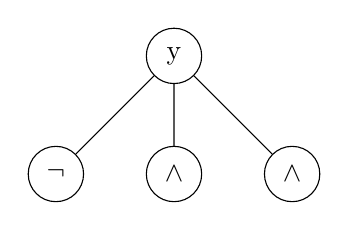
\begin{tikzpicture}[
            every node/.style = {minimum width = 2em, draw, circle},
        ]
        \node {y}
        child {node {$\neg$}}
        child {node {$\wedge$}}
        child {node {$\wedge$}};
    \end{tikzpicture}
}

Indeed, $w \in \lang$ iff then $C_{|w|}(w)=1$.
Therefore $\lang(C)=\lang$ and for each circuit in the ensemble $|C_n| = 0 \in O(1\}$ since there are no logic
gates in all the circuits in the ensemble.


\end{enumerate}


\bd{Bonus.} \\
In class we proved Myhill-Nerode's first direction: if a language has a DFA
accepting it, it has finitely many equivalence families.
We will now prove the second direction: if a language has finitely many
equivalence families, there is a DFA accepting it.
We have a language L with n equivalence families.

\begin{enumerate}[(a)]
      \item We will build a DFA $D = (Q, \AB, \de, q_0, F)$ accepting $\lang$:
We will denote the equivalence classes by $E_0=[x_0], E_1=[x_1], ... , E_{n-1}=x_{n-1}$,
where $x_0,...,x_{n-1}$ are different strings that 'represent' those classes.
The group of states, $Q$, will have a state per equivalence class, so $|Q|=n$
and $Q=\{[x_0],[x_1],...,x_{n-1}\}$, where $q_0=[x_0]=[\empw]$
and $F=\{[x_i] : \forall i \in \{0,...,n-1\} \text{ s.t. } [x_i] \subseteq \lang \}$. \\
The transition function will be:
\[
    \de([x_i], \ch) = [x_i \ch], \text{ } \forall i \in \{0,...,n-1\}, \ch \in \AB
\]



      \item We need to show that: $w \in \lang \Longleftrightarrow  w \in \lang(D)$. \\
First we show that:

Note that:

$ w \in \lang $ \\

$ \Longleftrightarrow \hat{\de}([x_0], w) \in F $ \\

$ \Longleftrightarrow  w \in \lang(D) $ \\
In conclusion, we got $w \in \lang \Longleftrightarrow  w \in \lang(N)$. Thus, concluding the proof. \\

We will define a state per equivalence class of $\lang$
transition function according to the equivalence class
accepting state if
\end{enumerate}


\end{document}